\subsection{Part 3}

The minimum cost of the system is 102 cost units. This cost
corresponds to 24 Micro Cell Channels at 1 cost unit per channel, and 78 Macro
Cell Channels at 3 cost units per channel.

The figure below shows the Total System cost versus the number of Micro Cell
channels. The cost decreases to 102 up to 24 Micro Cell Channels, and increases
past this value.

\begin{figure}[H]
	\centering
	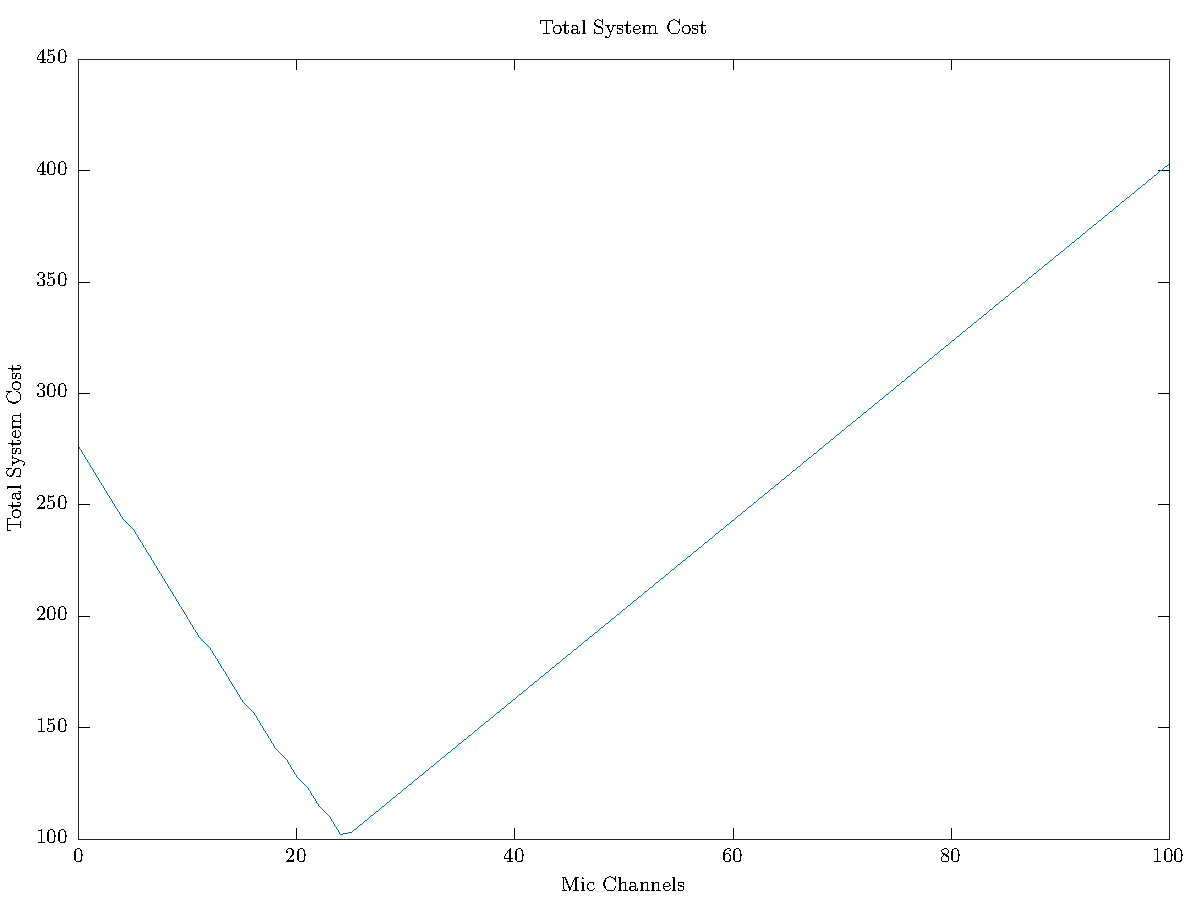
\includegraphics[width=0.8\textwidth]{code/Q6/Q6}
	\caption{Total System Cost vs. Micro Cell Channels}
	\label{fig:code-Q6-Q6}
\end{figure}

The following octave code shows the GNU-Octave implementation of the presented
problem. In order to calculate the minimum cost, the calculations described in
Part 2 are executed for increasing values of Micro Cell and Macro Cell Channels.
The blocking probability of each micro cell is calculated using the loops
current micro cell channel number and each cells respective offered load. These
blocking probabilities can be used to find the mean and variance for each cell.

A nested loop increments through the number of macro cell channels, calculating
the blocking probability, mean, and variance of the directly accessed macro
cell. The offered load and number of channels for the overflow channel is given
by using Rapps approximations on the total means and variances for the micro and
macro cells.

Using the offered load and number of channels for the overflow channel from
Rapps approximations, the overall blocking probability can be calculated. This
loop executes until the blocking probability drops below the required
QoS value of 1%.

For all calculations of blocking probabilities, the iterative method for
Erlang-B is used.

\lstinputlisting[language=octave]{code/Q6/q6.m}
